%% For double-blind review submission, w/o CCS and ACM Reference (max submission space)
\documentclass[acmsmall,review,anonymous]{acmart}\settopmatter{printfolios=true,printccs=false,printacmref=false}
%% For double-blind review submission, w/ CCS and ACM Reference
%\documentclass[acmsmall,review,anonymous]{acmart}\settopmatter{printfolios=true}
%% For single-blind review submission, w/o CCS and ACM Reference (max submission space)
%\documentclass[acmsmall,review]{acmart}\settopmatter{printfolios=true,printccs=false,printacmref=false}
%% For single-blind review submission, w/ CCS and ACM Reference
%\documentclass[acmsmall,review]{acmart}\settopmatter{printfolios=true}
%% For final camera-ready submission, w/ required CCS and ACM Reference
%\documentclass[acmsmall]{acmart}\settopmatter{}


%% Journal information
%% Supplied to authors by publisher for camera-ready submission;
%% use defaults for review submission.
\acmJournal{PACMPL}
\acmVolume{2}
\acmNumber{ICFP} % CONF = POPL or ICFP or OOPSLA
\acmArticle{1}
\acmYear{2018}
\acmMonth{9}
\acmDOI{10.1145/nnnnnnn.nnnnnnn}
\startPage{1}

%% Copyright information
%% Supplied to authors (based on authors' rights management selection;
%% see authors.acm.org) by publisher for camera-ready submission;
%% use 'none' for review submission.
\setcopyright{none}
%\setcopyright{acmcopyright}
%\setcopyright{acmlicensed}
%\setcopyright{rightsretained}
%\copyrightyear{2018}           %% If different from \acmYear

%% Bibliography style
\bibliographystyle{ACM-Reference-Format}
%% Citation style
%% Note: author/year citations are required for papers published as an
%% issue of PACMPL.
\citestyle{acmauthoryear}   %% For author/year citations


%%%%%%%%%%%%%%%%%%%%%%%%%%%%%%%%%%%%%%%%%%%%%%%%%%%%%%%%%%%%%%%%%%%%%%
%% Note: Authors migrating a paper from PACMPL format to traditional
%% SIGPLAN proceedings format must update the '\documentclass' and
%% topmatter commands above; see 'acmart-sigplanproc-template.tex'.
%%%%%%%%%%%%%%%%%%%%%%%%%%%%%%%%%%%%%%%%%%%%%%%%%%%%%%%%%%%%%%%%%%%%%%


%% Some recommended packages.
\usepackage{booktabs}   %% For formal tables:
                        %% http://ctan.org/pkg/booktabs
\usepackage{subcaption} %% For complex figures with subfigures/subcaptions
%% http://ctan.org/pkg/subcaption

\usepackage[utf8]{inputenc}
\usepackage[T1]{fontenc}
\usepackage[scaled=0.85]{beramono}
\usepackage{amsmath}
\usepackage{amssymb}
\usepackage{xcolor,colortbl}
\usepackage{url}
\usepackage{listings}
\usepackage{paralist}
\usepackage{wrapfig}
\usepackage{enumitem}
\usepackage{multicol}
\usepackage{flushend}
\usepackage{tikz}

\usetikzlibrary{arrows,chains,matrix,positioning,scopes}
\makeatletter
\tikzset{join/.code=\tikzset{after node path={%
\ifx\tikzchainprevious\pgfutil@empty\else(\tikzchainprevious)%
edge[every join]#1(\tikzchaincurrent)\fi}}}
\makeatother

\tikzset{>=stealth',every on chain/.append style={join},
         every join/.style={->}}
\tikzstyle{labeled}=[execute at begin node=$\scriptstyle,
   execute at end node=$]

% ----- listings

\definecolor{ckeyword}{HTML}{7F0055}
\definecolor{ccomment}{HTML}{3F7F5F}
\definecolor{cstring}{HTML}{2A0099}

\lstdefinelanguage{Scala}%
{morekeywords={abstract,%
  sealed,%
  case,catch,char,class,%
  def,else,extends,final,finally,for,%
  if,import,implicit,%
  match,module,%
  new,null,undefined,%
  fun,array,
  override,%
  package,private,protected,public,%
  for,public,return,super,%
  this,throw,trait,try,type,%
  val,var,%
  with,while,%
  let,skip,assert,then,fst,snd,root,idx,sum,prod,exists,forall,%
  yield%
  },%
  sensitive,%
  moredelim=*[il][\bfseries]{\#\#\ },
  morecomment=[l]//,%
  morecomment=[s]{/*}{*/},%
  morestring=[b]",%
%  morestring=[b]',%
  showstringspaces=false%
}[keywords,comments,strings]%

\lstset{language=Scala,%
  mathescape=true,%
%  columns=[c]fixed,%
%  basewidth={0.5em, 0.40em},%
%  aboveskip=5pt,%\smallskipamount,
%  belowskip=5pt,%\negsmallskipamount,
  lineskip=0pt,
  basewidth={0.54em, 0.4em},%
%  backgroundcolor=\color{listingbg},
  basicstyle=\footnotesize\ttfamily,
  keywordstyle=\keywordstyle,
  commentstyle=\commentstyle,
  stringstyle=\stringstyle,
%  xleftmargin=0.5cm
  literate={-->}{{$\to$}}3 
           {->}{{$\mapsto$}}3 
           {=>}{{$\Rightarrow$}}2 
           {|-}{{$\ts$}}2 
           %{fun}{{$\lambda$}}1 
           {idx}{{$\#$}}1 
           %{sum}{{$\Sigma$}}1 
           {array(}{{$\langle.\rangle$(}}3 
           %{[[}{{$[\![$}}1
           %{]]}{{$]\!]$}}1
           %{…}{{$\!...$}}1 
}

\definecolor{listingbg}{RGB}{240, 240, 240}

\newcommand{\commentstyle}[1]{\color{ccomment}\itshape{#1}}
\newcommand{\keywordstyle}[1]{\color{ckeyword}\bfseries{#1}}
\newcommand{\stringstyle}[1]{\color{cstring}\bfseries{#1}}

\lstnewenvironment{listing}{\lstset{language=Scala}}{}
\lstnewenvironment{listingtiny}{\lstset{language=Scala,basicstyle=\scriptsize\ttfamily}}{}

\newcommand{\code}[1]{\lstinline[language=Scala,columns=fixed,basicstyle=\ttfamily]|#1|}


\newcommand{\IMP}[0]{\texttt{IMP}}
\newcommand{\FUN}[0]{\texttt{FUN}}

\newcommand{\TOOL}[0]{\texttt{SIGMA}}



% ----- packed items, so we don't waste space
\newenvironment{sitemize}{
\begin{itemize}
  \setlength{\itemsep}{1pt}
  \setlength{\parskip}{0pt}
  \setlength{\parsep}{0pt}
}{\end{itemize}}

\newenvironment{senumerate}{
\begin{enumerate}
  \setlength{\itemsep}{1pt}
  \setlength{\parskip}{0pt}
  \setlength{\parsep}{0pt}
}{\end{enumerate}}

\newcommand{\mypar}[1]{{\bf #1.}}

% ----- formal

%\newcommand{\judgement}[2]{{\bf #1} \hfill #2}
%\newcommand{\den}[1]{$\left\llbracket$\;#1\;$\right\rrbracket$}
\newcommand{\den}[1]{\llbracket~#1~\rrbracket}

%\newcommand{\ts}{\,\vdash\,}
\newcommand{\evalsto}{\Downarrow}

\newcommand{\mbind}{\;{\small{\texttt{>>}\hspace{-0.3pt}\raisebox{-0.15pt}{\texttt{=}}}}\;}

%\newcommand{\mbind}{{\small{\texttt{>>}\hspace{-1.7pt}\raisebox{-0.15pt}{\texttt{=}}}}}

\newcommand{\rref}[1]{\textsc{(#1)}}

% ----- comments and todo

\newcommand{\note}[1]{{\color{red}[#1]}}
\newcommand{\todo}[1]{\note{TODO: #1}}

\newcommand{\silent}[1]{}



\lstMakeShortInline[keywordstyle=,%
                    flexiblecolumns=false,%
                    %basewidth={0.56em, 0.52em},%
                    mathescape=false,%
                    basicstyle=\tt]@

\begin{document}

%% Title information
\title{Pushdown Control-Flow Analysis via Refunctionalization (Functional Pearl)}         %% [Short Title] is optional;
                                        %% when present, will be used in
                                        %% header instead of Full Title.
%\titlenote{with title note}             %% \titlenote is optional;
                                        %% can be repeated if necessary;
                                        %% contents suppressed with 'anonymous'
\subtitle{Filling the Gap Between Abstracting Abstract Machines and Abstracting Definitional Interpreters}        %% \subtitle is optional
%\subtitlenote{with subtitle note}       %% \subtitlenote is optional;
                                        %% can be repeated if necessary;
                                        %% contents suppressed with 'anonymous'


%% Author information
%% Contents and number of authors suppressed with 'anonymous'.
%% Each author should be introduced by \author, followed by
%% \authornote (optional), \orcid (optional), \affiliation, and
%% \email.
%% An author may have multiple affiliations and/or emails; repeat the
%% appropriate command.
%% Many elements are not rendered, but should be provided for metadata
%% extraction tools.

%% Author with single affiliation.
\author{First1 Last1}
\authornote{with author1 note}          %% \authornote is optional;
                                        %% can be repeated if necessary
\orcid{nnnn-nnnn-nnnn-nnnn}             %% \orcid is optional
\affiliation{
  \position{Position1}
  \department{Department1}              %% \department is recommended
  \institution{Institution1}            %% \institution is required
  \streetaddress{Street1 Address1}
  \city{City1}
  \state{State1}
  \postcode{Post-Code1}
  \country{Country1}                    %% \country is recommended
}
\email{first1.last1@inst1.edu}          %% \email is recommended

%% Author with two affiliations and emails.
\author{First2 Last2}
\authornote{with author2 note}          %% \authornote is optional;
                                        %% can be repeated if necessary
\orcid{nnnn-nnnn-nnnn-nnnn}             %% \orcid is optional
\affiliation{
  \position{Position2a}
  \department{Department2a}             %% \department is recommended
  \institution{Institution2a}           %% \institution is required
  \streetaddress{Street2a Address2a}
  \city{City2a}
  \state{State2a}
  \postcode{Post-Code2a}
  \country{Country2a}                   %% \country is recommended
}
\email{first2.last2@inst2a.com}         %% \email is recommended
\affiliation{
  \position{Position2b}
  \department{Department2b}             %% \department is recommended
  \institution{Institution2b}           %% \institution is required
  \streetaddress{Street3b Address2b}
  \city{City2b}
  \state{State2b}
  \postcode{Post-Code2b}
  \country{Country2b}                   %% \country is recommended
}
\email{first2.last2@inst2b.org}         %% \email is recommended


%% Abstract
%% Note: \begin{abstract}...\end{abstract} environment must come
%% before \maketitle command
\begin{abstract}
  Abstracting abstract machines (AAM) is a systematic methodology 
  for constructing abstract interpreters that are derived from concrete
  small-step abstract machines. Recent progress applies the same idea 
  on definitional interpreter and obtains big-step 
  abstracting definitional interpreters (ADI) written in monadic style.
  Danvy shows the correspondence between concrete abstract machines and interpreters.
  Yet, the relations between small-step abstracting abstract machines and 
  big-step abstracting definitional interpreters is not well studied.

  In this paper, we show their correspondence and how to syntactically transform small-step 
  abstracting abstract machines into big-step abstracting definitional 
  interpreters.
  The transformations include fusing, disentangling, refunctionalizing 
  and monadification (or un-CPS to direct-style with delimited continuations). 
  All of them properly handle the 
  collecting semantics and the non-determinism of abstract interpretation. 
  After each transformation, we also obtain an intermediary form of 
  abstract interpreter.

  Following the idea that evaluation contexts are defunctionalized 
  continuations, we also found refunctionalization sequentializes the 
  non-deterministic abstract evaluation.
  Remarkably, we reveal how precise call/return match in control-flow 
  analysis can be obtained by properly refunctionalizing a small-step abstract interpreter.
  As well as we explain how it been lost by defunctionalizing the higher-order
  continuations into an first-order data type. 
  
  TODO: Maybe something Shiver's formulation of CFA in denotational style. 
 
\end{abstract}

%% 2012 ACM Computing Classification System (CSS) concepts
%% Generate at 'http://dl.acm.org/ccs/ccs.cfm'.
\begin{CCSXML}
<ccs2012>
<concept>
<concept_id>10011007.10011006.10011008</concept_id>
<concept_desc>Software and its engineering~General programming languages</concept_desc>
<concept_significance>500</concept_significance>
</concept>
<concept>
<concept_id>10003456.10003457.10003521.10003525</concept_id>
<concept_desc>Social and professional topics~History of programming languages</concept_desc>
<concept_significance>300</concept_significance>
</concept>
</ccs2012>
\end{CCSXML}

\ccsdesc[500]{Software and its engineering~General programming languages}
\ccsdesc[300]{Social and professional topics~History of programming languages}
%% End of generated code


%% Keywords
%% comma separated list
%\keywords{pushdown analysis, abstract interpretation, static analysis}  %% \keywords are mandatory in final camera-ready submission


%% \maketitle
%% Note: \maketitle command must come after title commands, author
%% commands, abstract environment, Computing Classification System
%% environment and commands, and keywords command.
\maketitle

\section{Introduction}

boardly speaking, AAM and ADI they are both abstract interpreters.

\subsection{Contributions}

the essence of abstracting definitional interpreter.

\begin{itemize}
\item The main contribution of this paper is we fill the gap
  between small-step AAM and big-step ADI by developing a series of
  systematic transformations. 
  The correspondence between abstract
  machines and interpreters exists not only in concrete semantics artifact,
  but also in abstract semantics artifact.
  Galois connection?

\item A new understanding of pushdown control-flow analysis by 
  refunctionalization.
  We present an abstract interpreter obtained from refunctionalizing
  an small-step abstracting abstract machine. 
  This abstract interpreter naturally enjoys pushdown control-flow property
  because the refunctionalization forces us to sequentialize the 
  abstract exectuion.
  We also analyze its correctness, soundness and termination.

\item Further, we show that defunctionalization and refunctionalization
  of abstract interpreters play important roles for call stack of analyzed language.
  Given this insight, we reveal that why small-step AAM has no pushdown
  control-flow property (if without extra efforts), as well as explain
  that why ADI naturally extends pushdown control-flow property from its
  defining language.

\end{itemize}

\subsection{Outline}

The paper is organized as follows. 

In section \ref{background}, we first describe the target language we will
analyze and a concrete CESK machine as operational semantics for it.
Then we review abstracting abstract machines (AAM) as an abstract interpretation
counterpart of CESK machines.

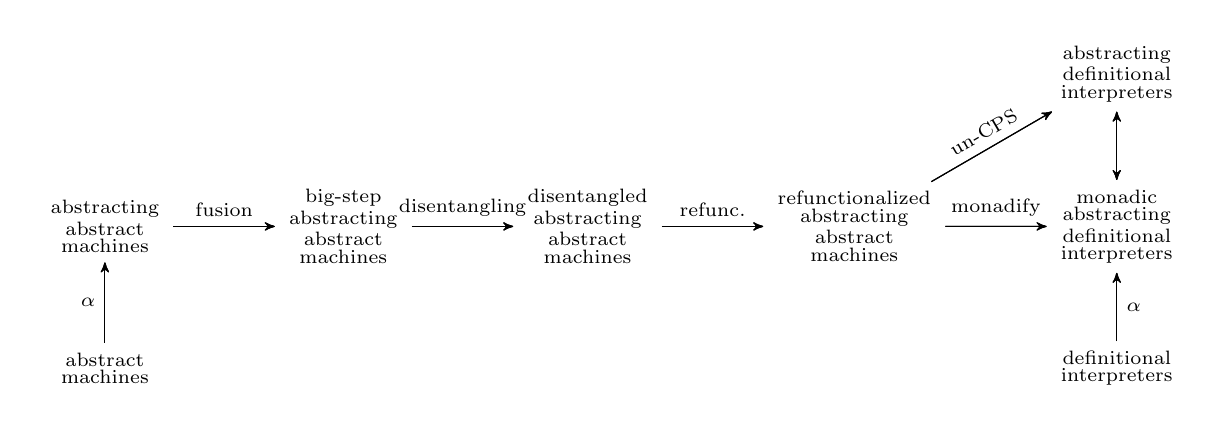
\begin{tikzpicture}
  \matrix (m) [matrix of math nodes, row sep=2.5em, column sep=3.7em]
    { 
        &  &  &  & 
      \begin{smallmatrix} \text{abstracting} \\ \text{definitional} \\ \text{interpreters} \end{smallmatrix} \\
      \begin{smallmatrix} \text{abstracting} \\ \text{abstract} \\ \text{machines} \end{smallmatrix} & 
      \begin{smallmatrix} \text{big-step} \\ \text{abstracting} \\ \text{abstract} \\ \text{machines} \end{smallmatrix}  & 
      \begin{smallmatrix} \text{disentangled}  \\ \text{abstracting} \\ \text{abstract} \\ \text{machines} \end{smallmatrix} & 
      \begin{smallmatrix} \text{refunctionalized}  \\ \text{abstracting} \\ \text{abstract} \\ \text{machines} \end{smallmatrix} & 
      \begin{smallmatrix} \text{monadic} \\ \text{abstracting} \\ \text{definitional} \\ \text{interpreters} \end{smallmatrix}  \\
      \begin{smallmatrix} \text{abstract} \\ \text{machines} \end{smallmatrix} & 
        &
      %\begin{smallmatrix} \text{big-step} \\ \text{abstract} \\ \text{machines} \end{smallmatrix}  & 
        &
      %\begin{smallmatrix} \text{disentangled} \\ \text{abstract} \\ \text{machines} \end{smallmatrix} & 
        &
      %\begin{smallmatrix} \text{refunctionalized} \\ \text{abstract} \\ \text{machines} \end{smallmatrix} & 
      \begin{smallmatrix} \text{definitional} \\ \text{interpreters} \end{smallmatrix} \\ 
    };
  {
    [start chain] \chainin (m-2-4);
    \chainin (m-1-5) [join={node[sloped,anchor=center,above,labeled] {\text{un-CPS}}}];
    \chainin (m-2-5) [join={node[above,labeled] {\text{}}}];
    \chainin (m-1-5) [join={node[above,labeled] {\text{}}}];
  }
  { 
    [start chain] \chainin (m-2-1);
    \chainin (m-2-2) [join={node[above,labeled] {\text{fusion}}}];
    \chainin (m-2-3) [join={node[above,labeled] {\text{disentangling}}}];
    \chainin (m-2-4) [join={node[above,labeled] {\text{refunc.}}}];
    \chainin (m-2-5) [join={node[above,labeled] {\text{monadify}}}];
  }
  { 
    [start chain] 
    \chainin (m-3-1);
    { [start branch=A] \chainin (m-2-1)
      [join={node[left, labeled] {\alpha}}];
    }
  }
    %\chainin (m-2-2);
    %\chainin (m-2-3);
    %\chainin (m-2-4);
  {
    [start chain] 
    \chainin (m-3-5); 
    { [start branch=B] \chainin (m-2-5)
      [join={node[right, labeled] {\alpha}}];
    }
  }
\end{tikzpicture}

\subsection{Style}

We use Scala language to demonstrate the idea and each step of transformations.
We expect that readers have moderate familiarity to Scala's syntax, such as
case classes, pattern matching and for comprehension.

There are two main reasons we use a real-world language:
1) The code does not diminish the accuracy of the material
than formal and mathematical notations, 
which are heavily used in other static analysis or semantics papers.
The Scala code in this paper can be easily back-translated into formal notations.
2) As a functional pearl, the code in this paper is executable with only few changes, 
which make it particularly fit for presenting syntactical transformations on abstract
interpreters.

\section{Background} \label{background}

\subsection{A-Normal Form $\lambda$-Calculus} \label{anfsyntax}

Traditionally, continuation-passing style (CPS) is a popular intermediate representation
for analyzing functional programs because of it exposes control transfer explicitly
and simplifies the analysis \cite{Shivers:1991:SSC:115865.115884, Shivers:1988:CFA:53990.54007}.
Here, we choose to use $\lambda$-calculus in administrative normal form (ANF) 
which is a direct-style intermediate representation as target for clarity 
but without losing simplicity and generality.
Although we just show the core calculus language, but it can be easily extended
to support recursive bindings (such as @letrec@), conditionals, primitive types and 
operations on primitive types. These cases would be trival or simple to implement, 
so we omit them in the paper.
The transformations we will show in the rest of this paper
also work on abstract machines for plain direct-style $\lambda$-calculus languages.

To begin, we now present the concrete syntax of a call-by-value $\lambda$-calculus language 
in ANF \cite{flanagan1993essence}.

\begin{lstlisting}
e $\in$ Exp ::= ae
          | (let ([x (ae ae)]) e)
ae $\in$ AExp ::= x            
            | lam
lam $\in$ Lam ::= (lambda (x) e)
x ... are variable names
\end{lstlisting}

In ANF, an expression is an atomic expression or a @let@ expression.
The restriction is all the function applications must be administrated in a @let@ expression,
and then bounded to a variable name under the current environment.
Both the operator and operand of function applications should be an atomic expression.
The atomic expressions $ae$ are either a variable, or a literal @lambda@ term, which
both can be evaluated in a single step.
We also assume that the program is globally alpha-renamed, i.e., all the
variable names are unique.

The abstract syntax can be straightforwardly described in Scala as follows:
TODO: update the abstract syntax.

\begin{lstlisting}
sealed trait Expr
case class Var(x: String) extends Expr
case class App(e1: Expr, e2: Expr) extends Expr
case class Lam(x: String, body: Expr) extends Expr
case class Let(x: String, e: App, body: Expr) extends Expr
\end{lstlisting}

\subsection{CESK Machine} \label{cesk}

\subsubsection{Machine Components}

\textit{C}ontrol \textit{E}nvionment \textit{S}tore \textit{K}ontinuation (CESK) machine is an
abstract machine for describing semantics of and evaluating $\lambda$-calculus \cite{felleisen1987calculus}.
CESK machine models program execution as state transitions in a small-step fashion. As its name suggested,
a machine state has four components: 1) Control is the expression currently being evaluated.
2) Environment is the a map that contains the address of a variable that in the lexical
scope of control.
3) Store models the heap of a program, and it is also a map but maps from addresses to values.
The addresses are infinite numbers starting from 0.
In our toy language, the only category of value is closure, i.e., a function paired with an environment.
4) Continuation represents the program stack.

We show the Scala representations for the components of CESK machine.

\begin{lstlisting}
type Addr = Int
type Env = Map[String, Addr]
type Store = Map[Addr, Storable]

abstract class Storable
case class Clos(v: Lam, env: Env) extends Storable

case class Frame(x: String, e: Expr, env: Env)
type Kont = List[Frame]

case class State(e: Expr, env: Env, store: Store, k: Kont)
\end{lstlisting}

It is worth noting that the continuation class @Kont@ is defined as a list of frames.
The frame class @Frame@ stores the information of call-site, i.e., the information that
can be used to resume the interrupted computation.
A @Frame@ constitutes of a variable name @x@ to be bind later, a control expression
that resumes to, and its environment. (TODO: mention that frame list vs KArg/KFun)

\subsubsection{Single-step Transition}
Before go into describing how the machine evaluates expressions, we firstly define several helper functions.
As we mentioned in section \ref{anfsyntax}, the atomic expressions are either a variable, or
a literal @lambda@ term. So the atomic expression evaluator @atomicEval@ handles these two
cases and evaluates atomic expressions to closures in a straightforward way.
The @alloc@ function generates a fresh address, and always allocates an unique integer under the domain
of store.
The @isAtomic@ function is used as a predicate of whether the expression is atomic.

\begin{lstlisting}
def atomicEval(e: Expr, env: Env, store: Store): Storable = e match {
  case Var(x) => store(env(x))
  case lam @ Lam(x, body) => Clos(lam, env)
}
def alloc(store: Store): Addr = store.keys.size + 1
def isAtomic(e: Expr): Boolean = e.isInstanceOf[Var] || e.isInstanceOf[Lam]
\end{lstlisting}

Now, we can faithfully describe the state transition function @step@,
that given a machine state, function @step@ determines its successor state.

\begin{lstlisting}
def step(s: State): State = s match {
  case State(Let(x, App(f, ae), e), env, store, k) if isAtomic(ae) =>
    val Clos(Lam(v, body), env_c) = atomicEval(f, env, store)
    val addr = alloc(store)
    val new_env = env_c + (v -> addr)
    val new_store = store + (addr -> atomicEval(ae, env, store))
    val frame = Frame(x, e, env)
    State(body, new_env, new_store, frame::k)
  case State(ae, env, store, k) if isAtomic(ae) =>
    val Frame(x, e, env_k)::ks = k
    val addr = alloc(store)
    val new_env = env_k + (x -> addr)
    val new_store = store + (addr -> atomicEval(ae, env, store))
    State(e, new_env, new_store, ks)
}
\end{lstlisting}

The first case is that the control of current state is a @Let@ expression,
and its right-hand side is an function application.
By calling evaluator @atomicEval@, we obtain the closure that callee @f@ stands for.
The successor state's control then transfers to the @body@ expression of closure,
with an updated environment and an update store. The new environment is extended
from closure's environment and mapped @v@ to a fresh address @addr@.
The new store is extended with @addr@ mapping to the value of @ae@,
which is evaluated from @atomicEval@.
In the meanwhile, a new frame @frame@ is pushed onto the stack @k@.
This @frame@ contains the variable name @x@ at left-hand side position of @Let@,
the body expression of @Let@, and the lexical environment of the body expression.

The second case for @step@ is the control is transferred to an atomic expression.
We extract the top frame of continuations firstly.
The control (that is an atomic expression) of current state is the evaluated term
that being bind to the variable @x@ from the top frame.
The environment and store are updated with @x@ mapping to the closure value of @ae@.
Then the successor state is transferred to expression @e@ from the top frame,
which is the body of a @Let@ expression, with the updated environment, store, and
the rest of stack @ks@.

\subsubsection{Valuation}

To run the program, we first use function @inject@ to construct an initial machine
state given an expression @e@. The initial state contains an empty environment, 
store and stack.
\begin{lstlisting}
def inject(e: Expr): State = State(e, Map(), Map(), Nil)
\end{lstlisting}

Then the @drive@ function is used to evaluate
to a final state by iteratively apply @step@ on current state until we reach a state
that the control is an atomic expression and the continuation stack is empty.
And of course, we can extract the value from the final state at last.

\begin{lstlisting}
def drive(s: State): State = s match {
  case State(ae, _, _, Nil) if isAtomic(ae) => s
  case _ => drive(step(s))
}
def eval(e: Expr): State = drive(inject(e))
\end{lstlisting}

\subsection{Abstracting Abstract Machine} \label{aam}
Abstracting abstract machine (AAM) is a systematic methodology that derives sound 
abstract interpreters for higher-order functional languages from concrete 
abstract machines \cite{van2012systematic, van2010abstracting}. 
An abstracting abstract machine implements computable abstract semantics that 
approximates the runtime behaviors of programs.
Since the state space of concrete execution is possibly infinite,
so to analyze programs, the key insight of AAM approach is to allocate both bindings
and continuations on the store, and then bound the addresses space to be finite.
Since each component of state is finite, 
thus the abstracted machine-state space is finite, and computable.

In this section, we derive the abstracting abstract machine from concrete
CESK machines, and also show that how to instantiate
useful $k$-call-sensitive control-flow analysis.

\subsubsection{Machine Components}

Similar with CESK machines, the machine state of AAM has a control expression,
an environment, a store and continuation, and in addition with a time-stamp.
But there are several notable differences of store between AAMs and concrete CESK machines.
In AAM, the store maps addresses to sets of values, so it stores all possible values
for a particular address. Thus the dereference an address becomes non-deterministic.
Also, the store performs a join rather than overwriting when updating elements of the store.
Third, the continuations are likewise allocated on store instead of formed a linked list,
and the continuation in a state then turns into a continuation address.

For clarity, we divide the store into binding store @BStore@ and continuation store @KStore@. 
The binding store maps binding addresses to sets of closure values, and continuation store maps
continuation addresses to sets of continuations.
We define a generic class @Store[K,V]@ that performs join when updating elements
in a store. By parameterizing @Store[K,V]@ with @[BAddr, Storable]@ and 
@[KAddr, Cont]@, we obtain @BStore@ and @KStore@, perspectively.

TODO(rephrase): Note that the store is monotonic, the store is always growing and never becoming 
smaller. This property guarantees we eventually will find a fixed point.

\begin{lstlisting}
case class Store[K,V](map: Map[K, Set[V]]) {
  def apply(addr: K): List[V] = map(addr).toList
  def update(addr: K, d: Set[V]): Store[K,V] = {
    val oldd = map.getOrElse(addr, Set())
    Store[K, V](map ++ Map(addr -> (d ++ oldd)))
  }
  def update(addr: K, sd: V): Store[K,V] = update(addr, Set(sd))
}
type BStore = Store[BAddr, Storable]
type KStore = Store[KAddr, Cont]
\end{lstlisting}

The co-domain of binding stores @Storable@ is the same
as we defined for CESK machines.
The co-domain of continuation stores @Cont@ is comprised of 
a frame @Frame@ and a continuation address @KAddr@.
To mimic the runtime call stack, @KAddr@ plays the role of
representing the remaining stack frames.
TODO: talk about nondet of cont deref?

\begin{lstlisting}
abstract class Storable 
case class Clos(v: Lam, env: Env) extends Storable

case class Frame(x: String, e: Expr, env: Env)
case class Cont(frame: Frame, kaddr: KAddr)
\end{lstlisting}

As a consequence, the components of a state is also changed: 
the store is divided into binding store and continuation store;
the continuation stack becomes an address.
By dereferencing this address in continuation store, we can retrieve the 
actual transfer of controls. The definition of environment @Env@
remains the same.

\begin{lstlisting}
case class State(e: Expr, env: Env, bstore: BStore, 
                 kstore: KStore, k: KAddr, time: Time)
\end{lstlisting}

\subsubsection{Allocating Addresses}
Up to now, we did not describe much about allocating adresses in stores and the 
time-stamp @Time@.
But in abstract interpretation, they are key ingredients to achieve 
analyses with different sensitivities, as well as to a finite state space analysis\cite{Gilray:2016:ACP:2951913.2951936}.
To effectively approximate the runtime behavior, a finite 
program contour @time@ that encodes the program execution history is introduced.
Here, we use a list of execution contexts (expressions) to represent that, and
as we will see in section \ref{kcfainst}, by applying different @tick@
functions to time we may obtain a family of analyses.

\begin{lstlisting}
type Time = List[Expr]
\end{lstlisting}

As we mentioned previously, the space of addresses has to be finite in AAM.
Binding addresses are parameterized by variable names and the time when creating this binding,
which are both finite.
Continuation addresses @KAddr@ has two variants: 
1) @Halt@ which corresponds to the empty stack, and
2) @ContAddr@ consists of the entry expressions of callee, which are also also
finite.
One may ask, why not also keep track of the time in continuation addresses?
(TODO: why target expression, allocation polyvariance)

\begin{lstlisting}
case class BAddr(x: String, time: Time)

abstract class KAddr
case object Halt extends KAddr
case class ContAddr(tgt: Expr) extends KAddr
\end{lstlisting}

We use two helper functions @allocBind@ and @allocKont@ that will be used later
to allocate binding addresses and continuation addresses.

\begin{lstlisting}
def allocBind(x: String, time: Time): BAddr = BAddr(x, time)
def allocKont(tgtExpr: Expr): KAddr = ContAddr(tgtExpr)
\end{lstlisting}

\subsubsection{Single-step Transition}

Since dereferencing an address becomes non-deterministic, our @atomicEval@
function also truns into non-deterministic. Given an atomic expression @e@,
@atomicEval@ returns a set of storable values, i.e., closures, to the caller.
If the expression is just a @lambda@ term, then the returned set is singleton.

\begin{lstlisting}
def atomicEval(e: Expr, env: Env, bstore: BStore): Set[Storable] = e match {
  case Var(x) => bstore(env(x))
  case lam@Lam(x, body) => Set(Clos(lam, env))
}
\end{lstlisting}

The structure of function @step@ is similar with concrete CESK machines, 
except non-determinism which makes @step@ returns a list of reachable 
successor states.
In the beginning of @step@, we call function @tick@ to update 
the time.
Then we have two cases to consider: 1) Current control expression is @Let@,
and @App(f, ae)@ is being bind to @x@.
Fristly we retrieve the set of closures that @f@ may represents.
For each closure in the set, we do almost the same as what we did in concrete 
CESK machines. But note that since the continuation is allocated on store (@kstore@),
a new continuation address @new_kaddr@ is constructed, and a new frame
@Frame(x, e, env)@ paired with the current continuation address @kaddr@
is joined into @new_kaddr@. Finally, a list of successors states is generated.

2) An atomic expression @ae@ sits on the control position of the state.
The value of @ae@ is being returned to its caller. 
We dereference the continuation address @kaddr@ and obtain a set of
continuations @conts@.
For each continuation in the set, we construct an environment based on the
environment of the frame (@env_f@), and bind @x@ to a newly created binding 
address @baddr@; also update the store with @baddr@ and 
the values that @ae@ represents. In every generated states,
the control becomes the expression @e@ in the frame,
and as we can tell from the name, continuation address @f_kaddr@
also comes from the frame.

\begin{lstlisting}
def step(s: State): List[State] = {
  val new_time = tick(s)
  s match {
    case State(Let(x, App(f, ae), e), env, bstore, kstore, kaddr, time) 
      if isAtomic(ae) =>
      val closures = atomicEval(f, env, bstore).toList
      for (Clos(Lam(v, body), env_c) <- closures) yield {
        val baddr = allocBind(v, new_time)
        val new_env = env_c + (v -> baddr)
        val new_bstore = bstore.update(baddr, atomicEval(ae, env, bstore))
        val new_kaddr = allocKont(body)
        val new_kstore = kstore.update(new_kaddr, Cont(Frame(x, e, env), kaddr))
        State(body, new_env, new_bstore, new_kstore, new_kaddr, new_time)
      }
    case State(ae, env, bstore, kstore, kaddr, time) 
      if isAtomic(ae) =>
      val conts = kstore(kaddr).toList
      for (Cont(Frame(x, e, env_f), f_kaddr) <- conts) yield {
        val baddr = allocBind(x, new_time)
        val new_env = env_f + (x -> baddr)
        val new_store = bstore.update(baddr, atomicEval(ae, env, bstore))
        State(e, new_env, new_store, kstore, f_kaddr, new_time)
      }
  }
}
\end{lstlisting}

\subsubsection{$k$-Call-Sensitive Instantiation} \label{kcfainst}

A histroy of last $k$ call sites is served as time information in
$k$-call-sensitive analysis.
The history is represented as a list of expressions and embedded
in the allocated addresses.

Every time when we transfer to next states, we use function @tick@ to
fresh the time and use this new time when allocating addresses. The function
@tick@ returns the $k$ front-most expressions given the current state and its
time history.

\begin{lstlisting}
def k: Int = 0
def tick(s: State): Time = (s.e :: s.time).take(k)
\end{lstlisting}

If we instantiate $k$ to be $0$, the history degenerates to an empty list,
then we obtain a monovariant analysis, which
not differentiates values at different call sites. In this case, the address
space collapses to the space of variable names.
Note that regarding to the ambiguitiy in
$k$-CFA\cite{Gilray:2016:ACP:2951913.2951936},
here the code actually implements a call+return sensitivity.

\subsubsection{Collecting Semantics}

To run (analyze) a program, as the CESK machines, we first use function @inject@ to construct
the initial state given the program. 
Note that the initial continuation store has a built-in mapping that maps continuation address
@Halt@ to empty set of continuations.
We also provide an empty program contour as initial time.
\begin{lstlisting}
def inject(e: Expr): State = 
  State(e, Map(), 
        Store[BAddr, Storable](Map()), 
        Store[KAddr, Cont](Map(Halt -> Set())), 
        Halt, List())
\end{lstlisting}

However, comparing with concrete CESK machine, the
@drive@ function performs collecting semantics instead of valuation
semantics. That is, for the purpose of analyzing programs, the function @drive@
collects all the intermediate machine states as the program is abstractly executing.
The following code shows a variant of work list algorithm to find the fixed-point 
of set of states.
Function @drive@ always applies function @step@ to the head element @hd@ of 
the work list @todo@ if @hd@ is unseen, then inserts the result of @step@ to 
the rest of work list; and in the meanwhile adds @hd@ to the explored states set.
If the work list is empty, the @drive@ just returns the set of reachable states 
up to now.

\begin{lstlisting}
def drive(todo: List[State], seen: Set[State]): Set[State] = todo match {
  case Nil => seen
  case hd::tl if seen.contains(hd) => drive(tl, seen)
  case hd::tl => drive(step(hd).toList ++ tl, seen + hd)
}

def analyze(e: Expr): Set[State] = drive(List(inject(e)), Set())
\end{lstlisting}

Finally, a user could use function @analyze@ to obtain all reachable states 
as a finite set for a given program.

%\subsection{Monadic Abstract Interpreter}
%Maybe not here?

\subsection{One Step Back: Unabstracted Stack}

In this section, we describe a variant of AAM that leaves stack to be 
unabstracted. That is to to use a precise call stack as we did in concrete CESK machine. 
Instead of allocating continuations on store and embedding
addresses of continuations in states, we intended to use a list of frames
to explicitly model the stack.
By doing so, we recover the call stack as precise as runtime 
(so called pushdown control-flow analysis), but since 
the stack is unbounded thus the analysis is possibly not computable.
For readers who do not familiarized pushdown analysis, we have a detailed 
discussion in Section \ref{pdcfarevisit}.
The reason we do so here is to establish an artifact with precise call/return match
used for the next step of transformation.

In the definition of state @State@, the continuation store disappears, and
component @konts@ becomes a list of frames. Other components keep the same.

\begin{lstlisting}
case class State(e: Expr, env: Env, bstore: BStore, konts: List[Frame], time: Time)
\end{lstlisting}

The state transition function @step@ shows in below which is still 
non-deterministic, but the only non-determinism happens when dereferencing the callee @f@ 
from function applications @App(f, ae)@. 

\begin{lstlisting}
def step(s: State): List[State] = {
  val new_time = tick(s)
  s match {
    case State(Let(x, App(f, ae), e), env, bstore, konts, time) if isAtomic(ae) =>
      for (Clos(Lam(v, body), env_c) <- atomicEval(f, env, bstore).toList) yield {
        val frame = Frame(x, e, env)
        val baddr = allocBind(v, new_time)
        val new_env = env_c + (v -> baddr)
        val new_store = bstore.update(baddr, atomicEval(ae, env, bstore))
        State(body, new_env, new_store, frame::konts, new_time)
      }
    case State(ae, env, bstore, konts, time) if isAtomic(ae) =>
      val Frame(x, e, env_f)::konts = konts
      val baddr = allocBind(x, new_time)
      val new_env = env_f + (x -> baddr)
      val new_store = bstore.update(baddr, atomicEval(ae, env, bstore))
      List(State(e, new_env, new_store, konts, new_time))
  }
}
\end{lstlisting}

In the first case of state matching, we may have multiple choices of closure for @f@.
For each closure in the set, a new frame is constructed and pushed onto the stack.
The code for handling the second case is the same as concrete CESK machines.
The function @drive@ should be also updated to prevent we pass a state with
empty frame list into function @step@.


\textbf{Note on Computability.}
Unfortunately, even though other components in states are finite, 
this AAM with unbounded stack is still not computable. 
Because the unbounded stack can grow to arbitrary deep which implies that the state space is possibly 
infinite, therefore the analysis may not terminate for all programs if we simply enumerating 
reachable states.
To see this, consider a program that has two mutually recursived functions:

\begin{lstlisting}
(letrec ([f1 (lambda (x) 
               (let ([x1 (f2 x)]) x1))]
         [f2 (lambda (y)
               (let ([y1 (f1 y)]) y1))])
  (let ([z (f1 1)])
    z))
\end{lstlisting}

Function @f1@ and @f2@ mutually invokes each others, and the stack will be 
alternatively pushing frame @f1@ and @f2@ onto the top of current stack, 
but not existing two stack components are identical in the state space.

\section{Fusing} \label{fusing}

In last section, we showed that by keeping an unabstracted stack in the state 
space we can recover the precise call/return match. In this section, we start
our first transformation: \textit{fusing} an AAM with unbounded-stack.

In fact, as later we will eliminate the stack and transform it to continuations
that are represented by higher-order functions, it does not matter what kind of 
AAM we start from. 
Because of transforming to higher-order functions forces us to sequentialize 
the order of abstract evaluation.
We choose to start from AAM with unbounded-stack just because it has a 
straightforward correspondence of pushdown semantics to refunctionalized AAM.

\begin{lstlisting}
def drive_step(todo: List[State], seen: Set[State]): Set[State] = todo match {
  case Nil => seen
  case hd::tl =>
    if (seen.contains(hd)) return drive_step(tl, seen)

    val new_time = tick(hd)
    val new_states = hd match {
      case State(Let(x, App(f, ae), e), env, bstore, konts, time) 
        if isAtomic(ae) =>
        for (Clos(Lam(v, body), env_c) <- atomicEval(f, env, bstore).toList) yield {
          val frame = Frame(x, e, env)
          val baddr = allocBind(v, new_time)
          val new_env = env_c + (v -> baddr)
          val new_store = bstore.update(baddr, atomicEval(ae, env, bstore))
          State(body, new_env, new_store, frame::konts, new_time)
        }
      case State(ae, env, bstore, konts, time) if isAtomic(ae) =>
        konts match {
          case Nil => List()
          case Frame(x, e, f_env)::konts =>
            val baddr = allocBind(x, new_time)
            val new_env = f_env + (x -> baddr)
            val new_store = bstore.update(baddr, atomicEval(ae, env, bstore))
            List(State(e, new_env, new_store, konts, new_time))
        }
    }
    drive_step(new_states ++ tl, seen + hd)
}

def analyze(e: Expr): Set[State] = drive_step(List(inject(e)), Set())
\end{lstlisting}

\section{Disentangling} \label{disen}

for plain direct-style, the continue function handles more cases.

\begin{lstlisting}
def aval(state: State, todo: List[State], seen: Set[State]): Set[State] = { 
  if (seen.contains(state)) return collect(todo, seen)

  val newTime = tick(state)
  state match {
    case State(Let(x, App(f, ae), e), env, bstore, konts, time) if isAtomic(ae) =>
      val newStates = for (Clos(Lam(v, body), c_env) <- atomicEval(f, env, bstore).toList) yield {
        val frame = Frame(x, e, env)
        val baddr = allocBind(v, newTime)
        val newEnv = c_env + (v -> baddr)
        val newStore = bstore.update(baddr, atomicEval(ae, env, bstore))
        State(body, newEnv, newStore, frame::konts, newTime)
      }   
      collect(newStates ++ todo, seen + state)
    case State(ae, env, bstore, konts, time) if isAtomic(ae) =>
      continue(konts, atomicEval(ae, env, bstore), bstore, newTime, todo, seen + state)
  }   
}

def collect(todo: List[State], seen: Set[State]): Set[State] = { 
  todo match {
    case Nil => seen
    case hd::tl => aval(hd, tl, seen)
  } 
}

def continue(konts: List[Frame], ds: Set[Storable], bstore: BStore, time: Time,
              todo: List[State], seen: Set[State]): Set[State] = konts match {
  case Nil => collect(todo, seen)
  case Frame(x, e, f_env)::konts =>
    val baddr = allocBind(x, time)
    val newEnv = f_env + (x -> baddr)
    val newStore = bstore.update(baddr, ds) 
    val newState = State(e, newEnv, newStore, konts, time)
    collect(newState::todo, seen)
}

def analyze(e: Expr): Set[State] = aval(inject(e), List(), Set()) 
\end{lstlisting}

\section{Refunctionalization} \label{refunc}

As we pointed earlier, refunctionalizing evaluation contexts to higher-order
continuation functions forces us to somehow sequentialize the abstract evaluation.
We identify that in order to sequentialize abstract evaluation, there are three
fundamental differences with concrete evaluation: 
1) The dereferencing store addresses is non-deterministic, therefore the returning
may also be non-deterministic.
2) We need sound collecting semantics rather than valuation semantics.
3) The abstract evaluation has to be terminating.

allocating continuations of defined language on the heap of defining language.

\subsection{First Try}

Transform to Extended Continuation-Passing Style (ECPS), continuation and meta-continuation.
simply trun evaluation contexts into higher-order continuations.
We establish pushdown control-flow, but this is not computable.

\begin{lstlisting}
case class VS(vals: Set[Storable], time: Time, store: BStore)
type NCont = Set[VS] => Set[VS]
type Cont  = NCont => (Set[VS] => Set[VS])

def aval(e: Expr, env: Env, store: BStore, time: Time,
          cont: Cont, ncont: NCont): Set[VS] = {
  val new_time = (e::time).take(k)
  e match {
    case Let(x, App(f, ae), e) =>
      val closures = aeval(f, env, store).toList.asInstanceOf[List[Clos]]

      def new_ncont(ret_vss: Set[VS])(result: Set[VS]): Set[VS] = {
        val VS(vals, time, store) = ret_vss.head
        val baddr = allocBind(x, time)
        val new_env = env + (x -> baddr)
        val new_store = store.update(baddr, vals)
        aval(e, new_env, new_store, time, (r: NCont) => r, (vss1: Set[VS]) => {
          if (ret_vss.tail.isEmpty) cont(ncont)(result ++ vss1)
          else new_ncont(ret_vss.tail)(result ++ vss1)
        })
      }

      def nd(closures: List[Clos], vss_acc: Set[VS]): Set[VS] = {
        val Clos(Lam(v, body), c_env)::rest = closures
        val baddr = allocBind(v, new_time)
        val new_env = c_env + (v -> baddr)
        val new_store = store.update(baddr, aeval(ae, env, store))
        aval(body, new_env, new_store, new_time, (r: NCont) => r, (vss: Set[VS]) => {
          if (rest.isEmpty) new_ncont(vss_acc ++ vss)(Set())
          else nd(rest, vss_acc ++ vss)
        })
      }

      nd(closures, Set())

    case ae if isAtomic(ae) =>
      val ds = aeval(ae, env, store)
      cont(ncont)(Set(VS(ds, new_time, store)))
  }
}

def mtTime = List()
def mtEnv = Map[String, BAddr]()
def mtStore = Store[BAddr, Storable](Map())

def analyze(e: Expr) = aval(e, mtEnv, mtStore, mtTime, 
                            (r: NCont) => (vss: Set[VS]) =>  r(vss), 
                            (vss: Set[VS]) => vss)
\end{lstlisting}

\subsection{Caching Fixed-Points}

fix point cache

\begin{lstlisting}
\end{lstlisting}

\subsection{Pushdown Control-Flow Analysis, Revisited} \label{pdcfarevisit}

Pushdown control-flow is a property in analysis that precisely models
the runtime call-stack of the analyzed program. 
A pushdown control-flow analysis provides as exact as runtime return-flow 
when analyzing the program, but traditional control-flow analysis collapses 
the state space into a finite space thus causes imprecise stack modeling.

To see how traditional CFA suffers from spurious return-flows, 
we can consider the following example:

\begin{lstlisting}
(let ([id (lambda (z) z)])
  (let ([x (id 1)])
    (let ([y (id 2)])
      x)))
\end{lstlisting}

In traditional $k$-CFA algorithm and the AAM we showed in section \ref{aam}, 
the return-flow of invocation @(id 2)@
is going to both call-sites @(id 1)@ and @(id 2)@. Therefore, the
returned value @2@ for variable @y@ is also propagated to 
variable @x@ and then imprecise analysis result is arose.
This return-flow merging is inevitable even we increase the context-sensitivity.
If we use the monovariant analysis (i.e. 0CFA), the analyzing result would be @x@ and 
@y@ point to set @{1, 2}@, because the algorithm not distinguishes
@z@ comes from different call-sites.
Under $1$-CFA, the algorithm is able to distinguish that variable @z@ of function
@id@ has two different values at two call-sites, so variable @y@ 
would not be polluted by @1@. 
But two call-sites still share the same continuation and
it is still helplessness for separating the return-flows.
TODO: do need more details to explain this example? (as in P4F paper)

%probably Store Widening \& Abstract Garbage Collection
\section{To Direct-Style}

In previous section, we presented a refunctionalized AAM that in extended continuation-passing style. 
To obtain a definitional abstract interpreter, we need to transform it further to direct-style. 
At this point, we have two choices: 
1) By monadifying the continuations into monads, we obtain the \citeauthor{darais2017abstracting}'s 
abstracting definitional interpreter in monadic style.
2) By representing the extended continuation-passing style with delimited continuations,
we derive a new form of abstract interpreters in direct-style.
This coincidence should not be a surprise since there are extraordinarily rich literatures 
show the correspondence between monads and continuations as of their very beginning era
(TODO: cite Danvy/abs control/esce of fp).
In fact, we can also just use the same caching algorithm but with side effect such as 
assignments and mutations to achieve the same definitional interpreter with pushdown
control flows.
In this section, we present both of versions using monads and delimited controls.

\subsection{Monadification} \label{monadify}

In this section, we show how to transform the refunctionalized AAM to monadic-style
abstracting definitional interpreters.

\subsection{Un-CPS} \label{uncps}

On another path, here, we introduce direct-style abstracting definitional interpreter 
with delimited control operators @reset@ and @shift@.

TODO: This version does not use delimited controls.

\begin{lstlisting}
def aval(e: Expr, env: Env, store: BStore, time: Time, cache: Cache): (Set[VS], Cache) = {
  val config = Config(e, env, time)
  if (cache.outContains(config)) return (cache.outGet(config), cache)

  val new_cache = cache.outUpdate(config, cache.inGet(config))
  val new_time = (e::time).take(k)

  e match {
    case Let(x, App(f, ae), e) =>
      val closures = aeval(f, env, store).toList.asInstanceOf[List[Clos]]
      val app_vss_cache = for (Clos(Lam(v, body), c_env) <- closures) yield {
        val baddr = allocBind(v, new_time)
        val new_env = c_env + (v -> baddr)
        val new_store = store.update(baddr, aeval(ae, env, store))
        aval(body, new_env, new_store, new_time, new_cache) //TODO: Do we have to use the latest cache?
      }

      val app_vss = app_vss_cache.map(_._1).foldLeft(Set[VS]())(_ ++ _)
      val app_cache = app_vss_cache.map(_._2).foldLeft(mtCache)(_.outJoin(_))

      val e_vss = for (VS(vals, time, store) <- app_vss.toList) yield {
        val baddr = allocBind(x, time)
        val new_env = env + (x -> baddr)
        val new_store = store.update(baddr, vals)
        aval(e, new_env, new_store, time, app_cache) //TODO: Do we have to use the latest cache?
      }
      val result = e_vss.map(_._1).foldLeft(Set[VS]())(_ ++ _)
      (result, e_vss.map(_._2).foldLeft(mtCache)(_.outJoin(_)).outUpdate(config, result))

    case ae if isAtomic(ae) =>
      val ds = aeval(ae, env, store)
      (Set(VS(ds, new_time, store)), new_cache.outUpdate(config, VS(ds, new_time, store)))
  }
}

def analyze(e: Expr) = {
  def iter(cache: Cache): (Set[VS], Cache) = {
    val (vss, new_cache) = aval(e, mtEnv, mtStore, mtTime, cache)
    if (new_cache.out == cache.out) (vss, new_cache)
    else iter (Cache(new_cache.out, new_cache.out))
  }
  iter(mtCache)
}
\end{lstlisting}

\section{Refunctionalized AAM}

May be insert to section refunc.

\subsection{Store Widening}

\subsection{Higher-Order Controls?}

TODO: analyze programs with call/cc, shift, reset.

\subsection{Precise Call/Return Match}

show the precision of stack

On equivalence: since refunc interp does not have an explicit concept of $state$,
so 1) we can compare the final states of P4F against with refunc interp,
or 2) we can compare the summarized store of P4F against with summarized store of refunc interp.

\subsection{Termination}

show that number of continuation is finite.

\subsection{Soundness}

\subsection{Complexity}

\section{Perspective}

\subsection{Defunctionalization}

specify higher-order definitional interpreters using first-order means (cite)

\subsection{Refunctionalization}

%\section{Detour: Shiver's \textit{k}-CFA?}

\section{Related Work}

\textbf{Pushdown Control-flow Analysis}
In recent years, there are significant efforts \cite{vardoulakis2010cfa2, earl2012introspective, 
gilray2016pushdown, johnson2015abstracting} to achieve precise call/return 
match based on small-step AAM which is what we described in section \ref{aam}.

CFA2 is the first solution that solves the return-flows problem\cite{vardoulakis2010cfa2}.
But CFA2 has several drawbacks: it works on only continuation-passing style programs, 
and not supports polyvariant analysis, in addition with an exponential time complexity.
TODO: summarize PDCFA, AAC

\citeauthor{gilray2016pushdown} proposed a polyvariant address allocator for continuations
under small-step abstracting abstract machines that is both simple to implement and
computational inexpensive. 
Based on the AAM we presented in Section \ref{aam}, the only change in code is
not only keeping track of the entry-point expression of callee, but also holding the target environment
when allocating a continuation address.
The target environment is the binding environment extended from closure's environment
(namely @val new_env = env_c + (v -> baddr)@). All the other part of the code remain the same.
The following code shows the implementation:

\begin{lstlisting}
case class P4FContAddr(tgt: Expr, tgtEnv: Env) extends KAddr
def allocKont(tgtExpr: Expr, tgtEnv: Env): KAddr = P4FContAddr(tgtExpr, tgtEnv)
\end{lstlisting}

TODO: explain the reason why it works.

Notably, this change only causes constant-factor increase in time complexity of 
the analysis if the store is widened.

TOOD: why only needs the target env. correspondence?

\textbf{Abstracting Definitional Interpreters.}
On the other side of small-step AAM, with the insight from Reynold's seminal paper 
\emph{Definitional interpreters for higher-order programming languages} \cite{reynolds1972definitional}
that the defined language will inherit properties from the defining language, 
\citeauthor{darais2017abstracting} construct abstracting 
definitional interpreters that automatically inherit the pushdown control-flow 
property from its defining language.

\citeauthor{darais2017abstracting}'s abstracting definitional interpreters is written
in monadic style.

composable.
TODO: connection to this paper.
TODO: although they establish pushdown control-flow analysis in different ways, 
is there a correspondence between different methods?

\textbf{Defunctionalization and Refunctionalization.}

\section{Conclusion}

%% Acknowledgments
\begin{acks}                            %% acks environment is optional
                                        %% contents suppressed with 'anonymous'
  %% Commands \grantsponsor{<sponsorID>}{<name>}{<url>} and
  %% \grantnum[<url>]{<sponsorID>}{<number>} should be used to
  %% acknowledge financial support and will be used by metadata
  %% extraction tools.
  This material is based upon work supported by the
  \grantsponsor{GS100000001}{National Science
    Foundation}{http://dx.doi.org/10.13039/100000001} under Grant
  No.~\grantnum{GS100000001}{nnnnnnn} and Grant
  No.~\grantnum{GS100000001}{mmmmmmm}.  Any opinions, findings, and
  conclusions or recommendations expressed in this material are those
  of the author and do not necessarily reflect the views of the
  National Science Foundation.
\end{acks}

%% Bibliography
\bibliography{references}

%% Appendix
\appendix
\section{Appendix}

Text of appendix \ldots

\end{document}
